\documentclass[a4paper, 11pt]{article}
\usepackage{comment} % enables the use of multi-line comments (\ifx \fi) 
\usepackage{lipsum} %This package just generates Lorem Ipsum filler text. 
\usepackage{fullpage} % changes the margin
\usepackage{graphicx}
\graphicspath{.}

\begin{document}
%Header-Make sure you update this information!!!!
\noindent
\LARGE\textbf{AML HW8 EM Algorithm} \\
\large\textbf{Yu Che Wang / yuchecw2} \\

\section{Tree segmented images}
\begin{figure}[h!]
\centering
    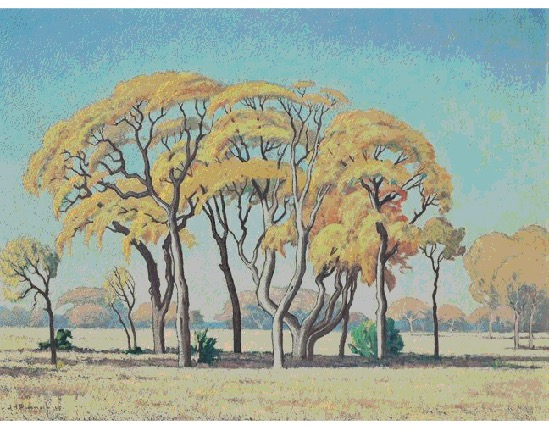
\includegraphics[width=7.5cm, height=5cm]{images/Tree_10.jpeg}
    \caption{Tree image with 10 segments}
\end{figure}
\begin{figure}[h!]
\centering
    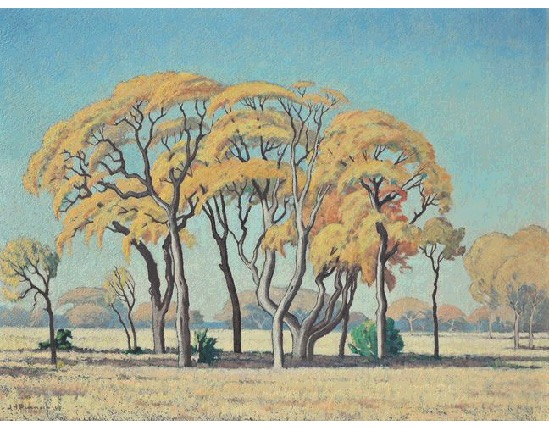
\includegraphics[width=7.5cm, height=5cm]{images/Tree_20.jpeg}
    \caption{Tree image with 20 segments}
\end{figure}
\begin{figure}[h!]
\centering
    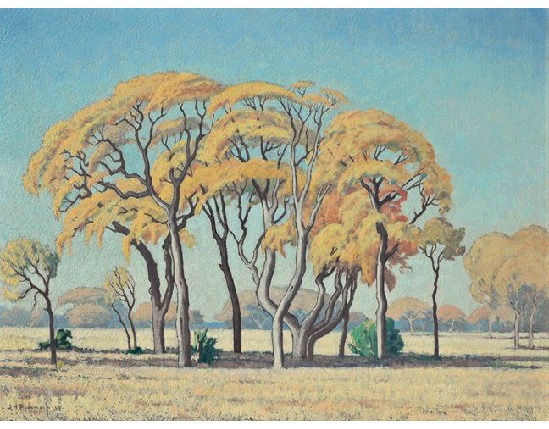
\includegraphics[width=7.5cm, height=5cm]{images/Tree_50.jpeg}
    \caption{Tree image with 50 segments}
\end{figure}
\clearpage

\section{RobertMixed segmented images}
\begin{figure}[h!]
\centering
    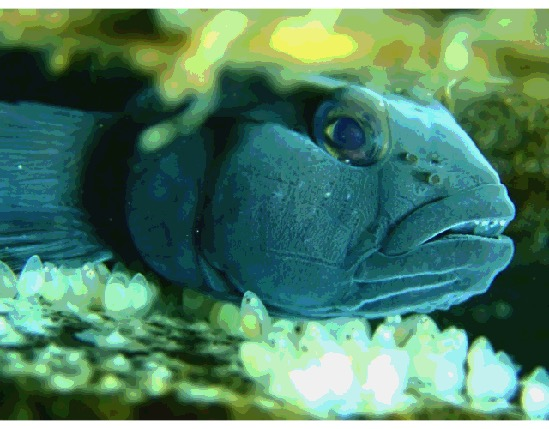
\includegraphics[width=7.5cm, height=5cm]{images/Fish_10.jpeg}
    \caption{RobertMixed image with 10 segments}
\end{figure}
\begin{figure}[h!]
\centering
    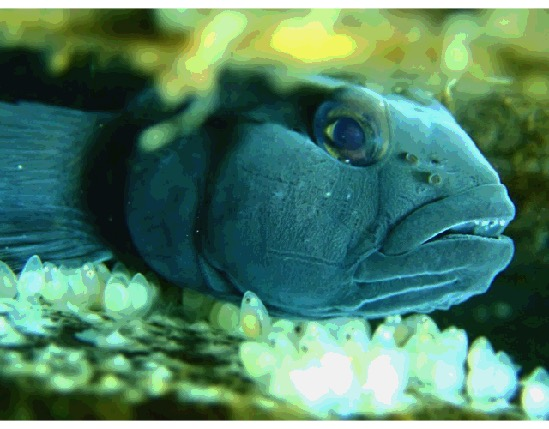
\includegraphics[width=7.5cm, height=5cm]{images/Fish_20.jpeg}
    \caption{RobertMixed image with 20 segments}
\end{figure}
\begin{figure}[h!]
\centering
    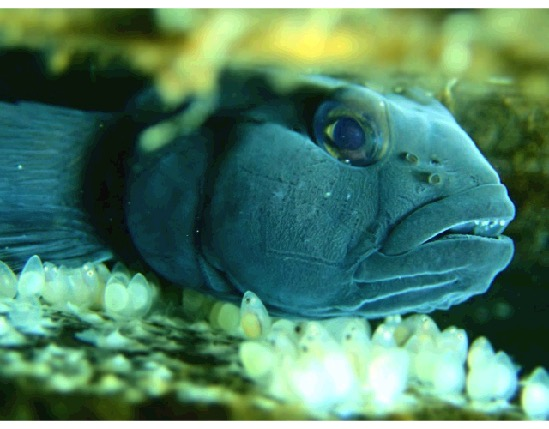
\includegraphics[width=7.5cm, height=5cm]{images/Fish_50.jpeg}
    \caption{RobertMixed image with 50 segments}
\end{figure}
\clearpage

\section{Strelitzia segmented images}
\begin{figure}[h!]
\centering
    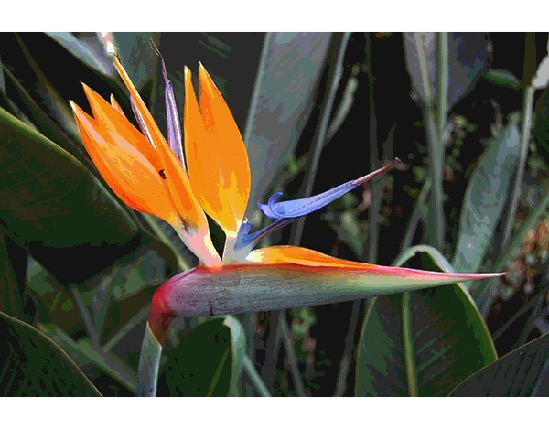
\includegraphics[width=7.5cm, height=5cm]{images/S_10.jpeg}
    \caption{Strelitzia image with 10 segments}
\end{figure}
\begin{figure}[h!]
\centering
    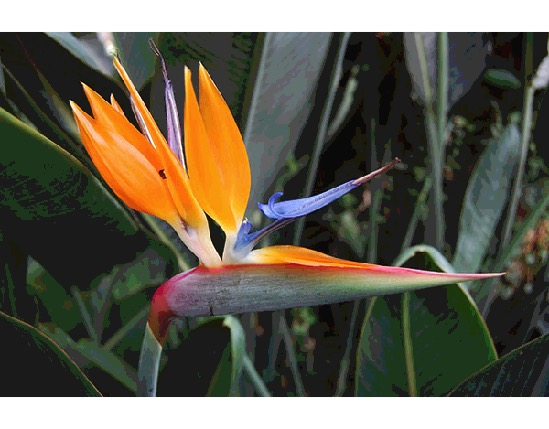
\includegraphics[width=7.5cm, height=5cm]{images/S_20.jpeg}
    \caption{Strelitzia image with 20 segments}
\end{figure}
\begin{figure}[h!]
\centering
    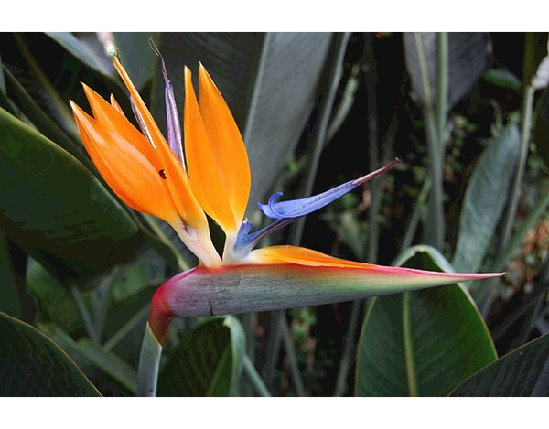
\includegraphics[width=7.5cm, height=5cm]{images/S_50.jpeg}
    \caption{Strelitzia image with 50 segments}
\end{figure}
\clearpage

\section{Sunset segmented images}
\begin{figure}[h!]
\centering
    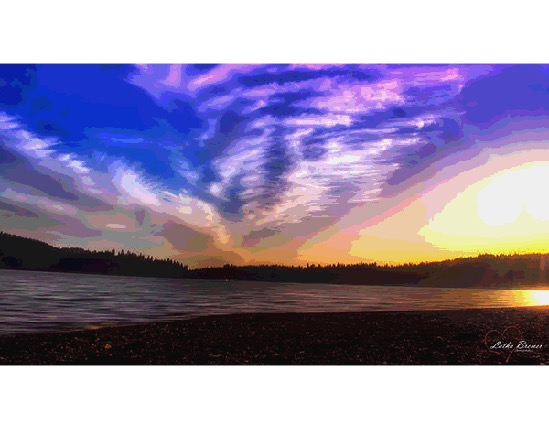
\includegraphics[width=7.5cm, height=5cm]{images/Sunset_10.jpeg}
    \caption{Sunset image with 10 segments}
\end{figure}
\begin{figure}[h!]
\centering
    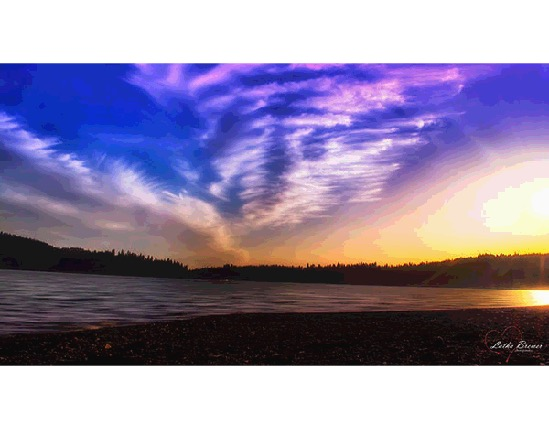
\includegraphics[width=7.5cm, height=5cm]{images/Sunset_20.jpeg}
    \caption{Sunset image with 20 segments}
\end{figure}
\begin{figure}[h!]
\centering
    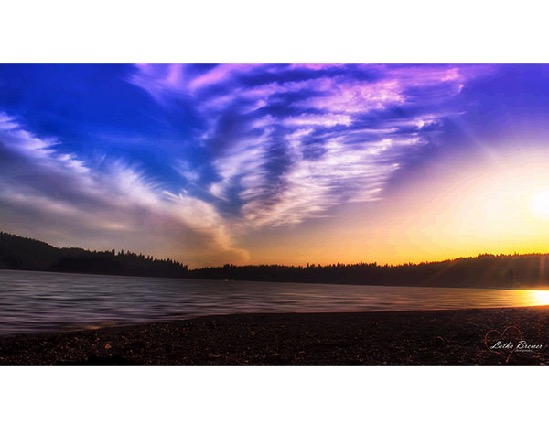
\includegraphics[width=7.5cm, height=5cm]{images/Sunset_50.jpeg}
    \caption{Sunset image with 50 segments}
\end{figure}
\clearpage

\section{Tree segmented images with different starting points}
\begin{figure}[h!]
\centering
    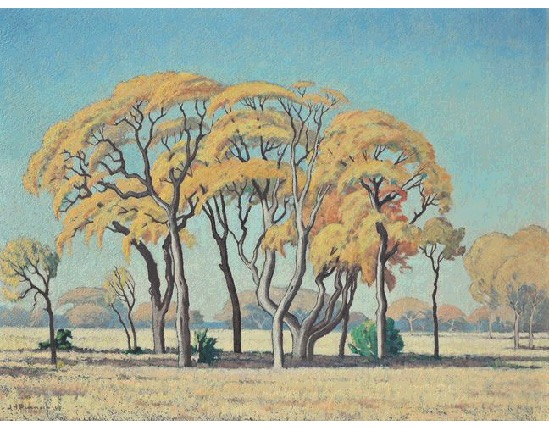
\includegraphics[width=6cm, height=4cm]{images/Tree_20.jpeg}
    \caption{Tree-1}
\end{figure}
\begin{figure}[h!]
\centering
    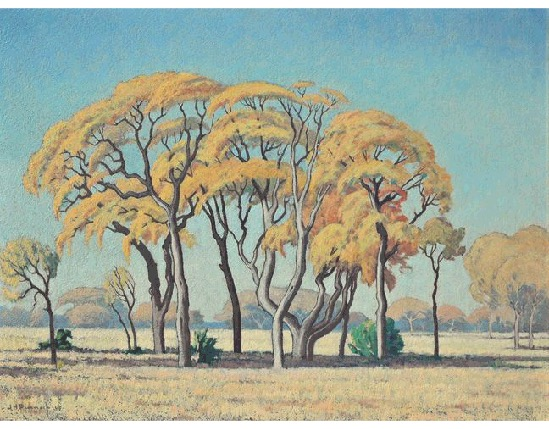
\includegraphics[width=6cm, height=4cm]{images/Tree_20_1.jpeg}
    \caption{Tree-2}
\end{figure}
\begin{figure}[h!]
\centering
    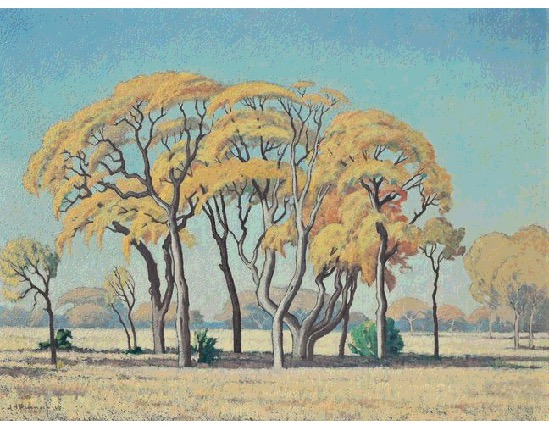
\includegraphics[width=6cm, height=4cm]{images/Tree_20_2.jpeg}
    \caption{Tree-3}
\end{figure}
\begin{figure}[h!]
\centering
    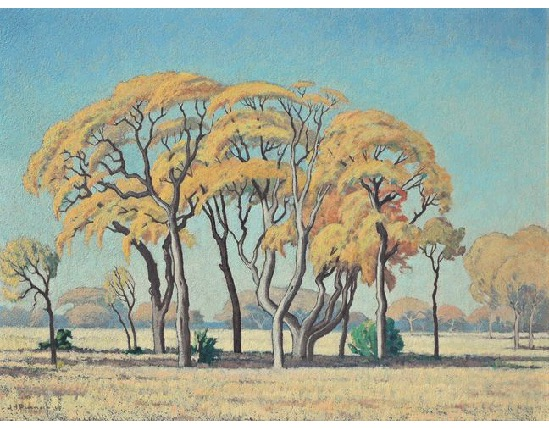
\includegraphics[width=6cm, height=4cm]{images/Tree_20_3.jpeg}
    \caption{Tree-4}
\end{figure}\begin{figure}[h!]
\centering
    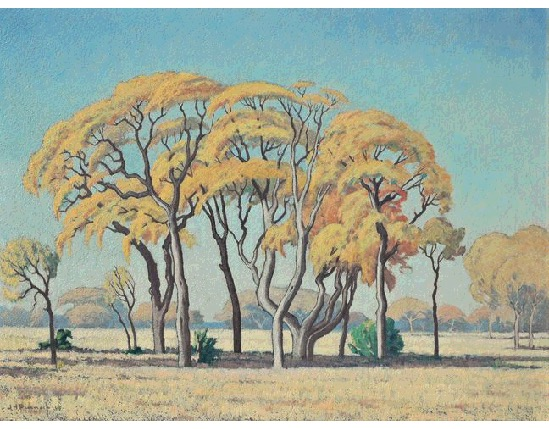
\includegraphics[width=6cm, height=4cm]{images/Tree_20_4.jpeg}
    \caption{Tree-5}
\end{figure}


\section{Code snippets for EM initialization and updates}
\begin{figure}[h!]
\centering
    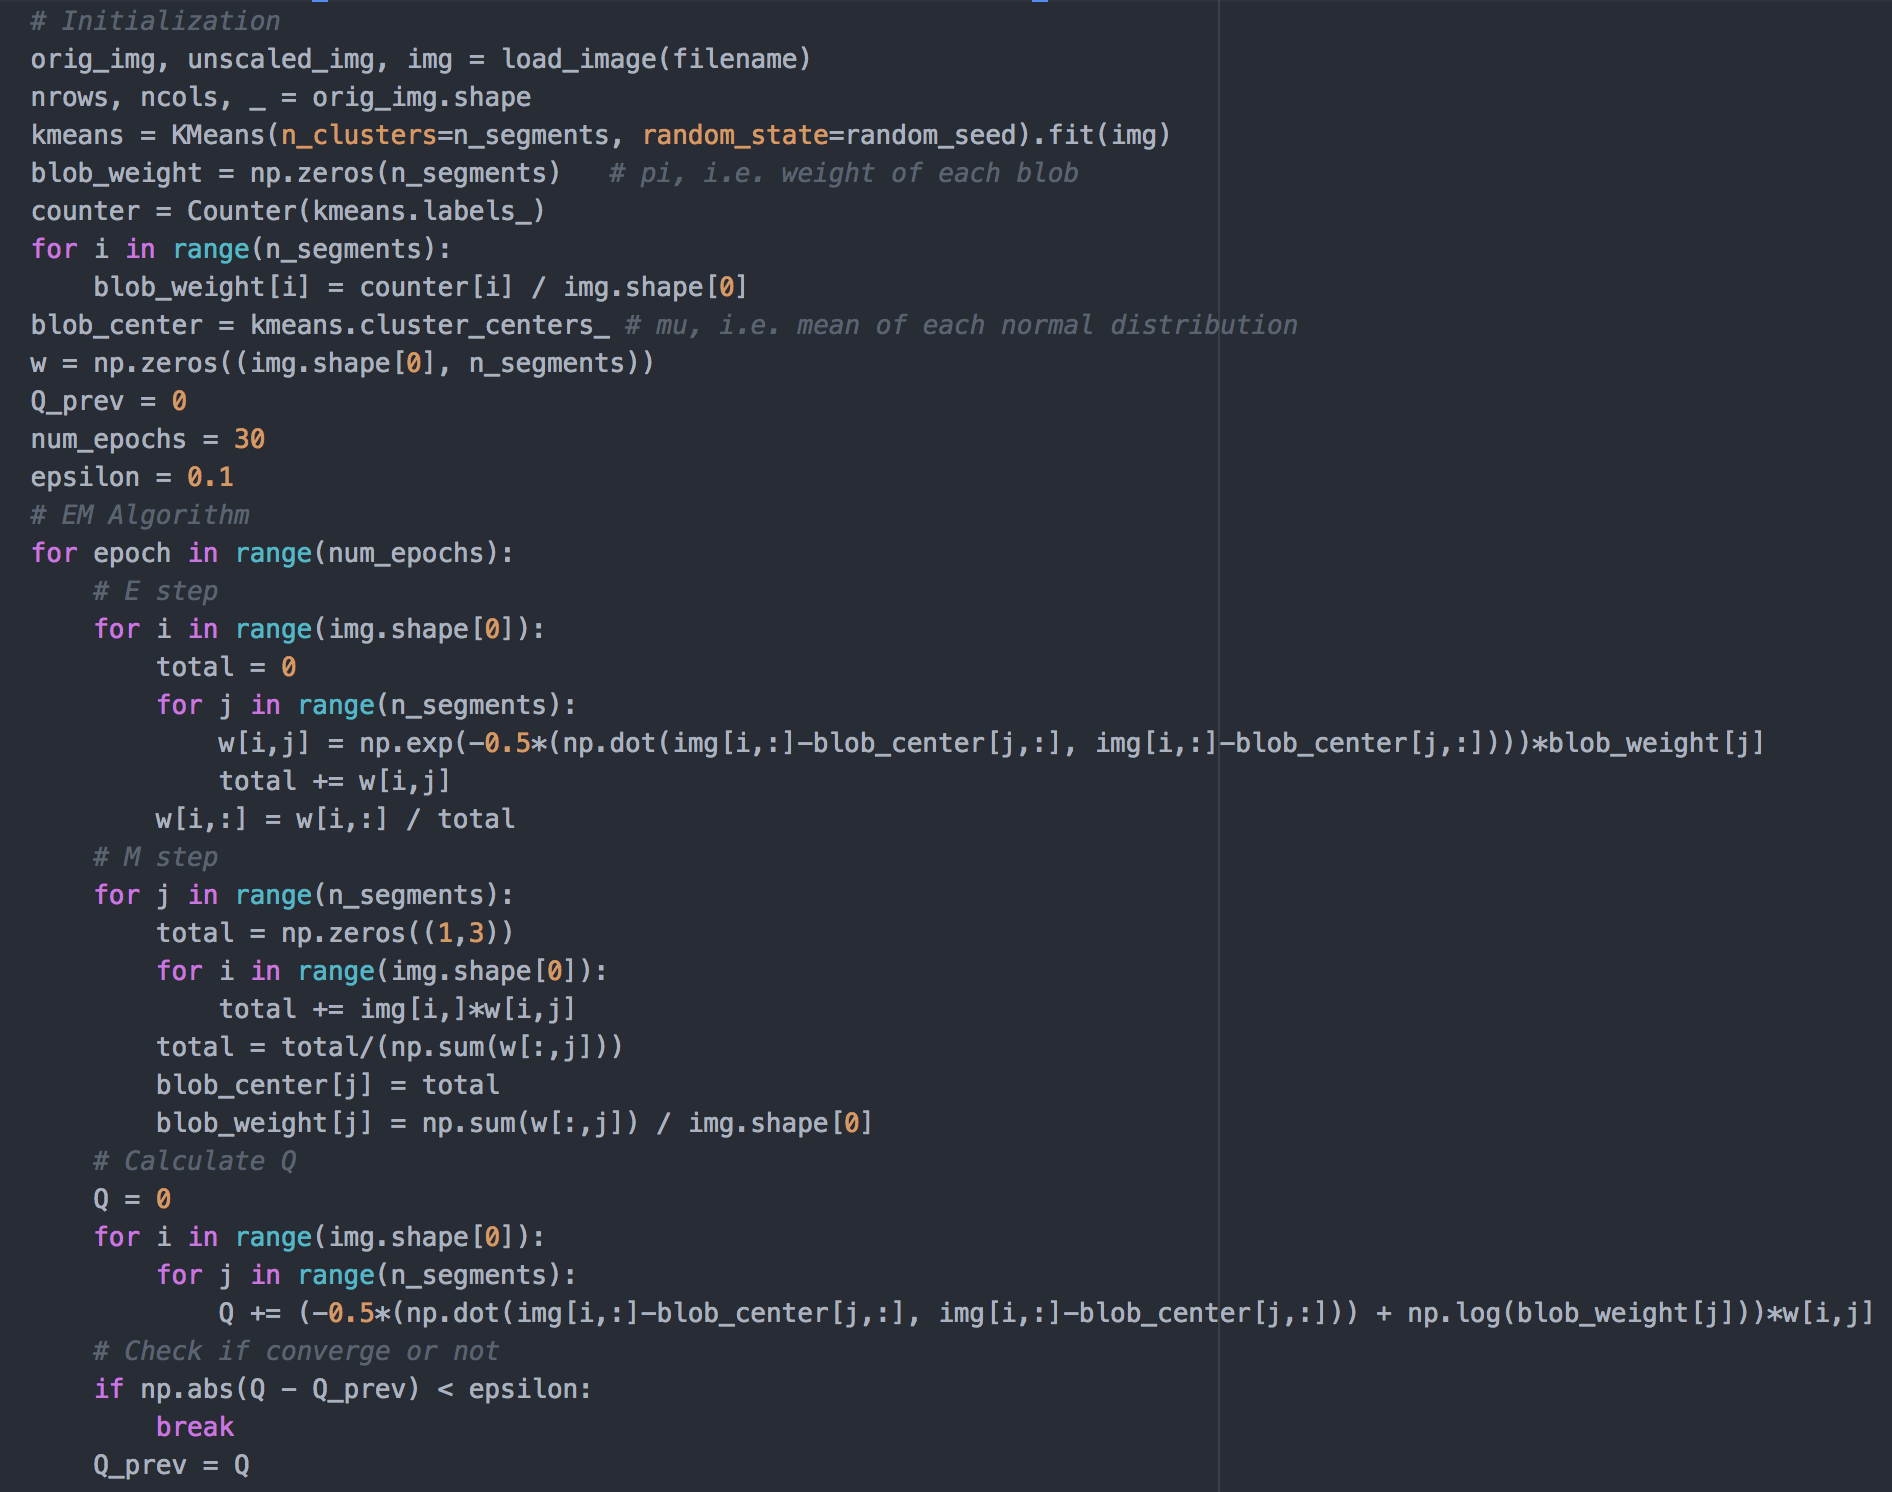
\includegraphics[width=17cm, height=12cm]{images/code.jpeg}
    \caption{Code snippets}
\end{figure}
\end{document}

